\section{SwitchBox Design}\label{sec:design}

\begin{figure}[t]
   \centering
   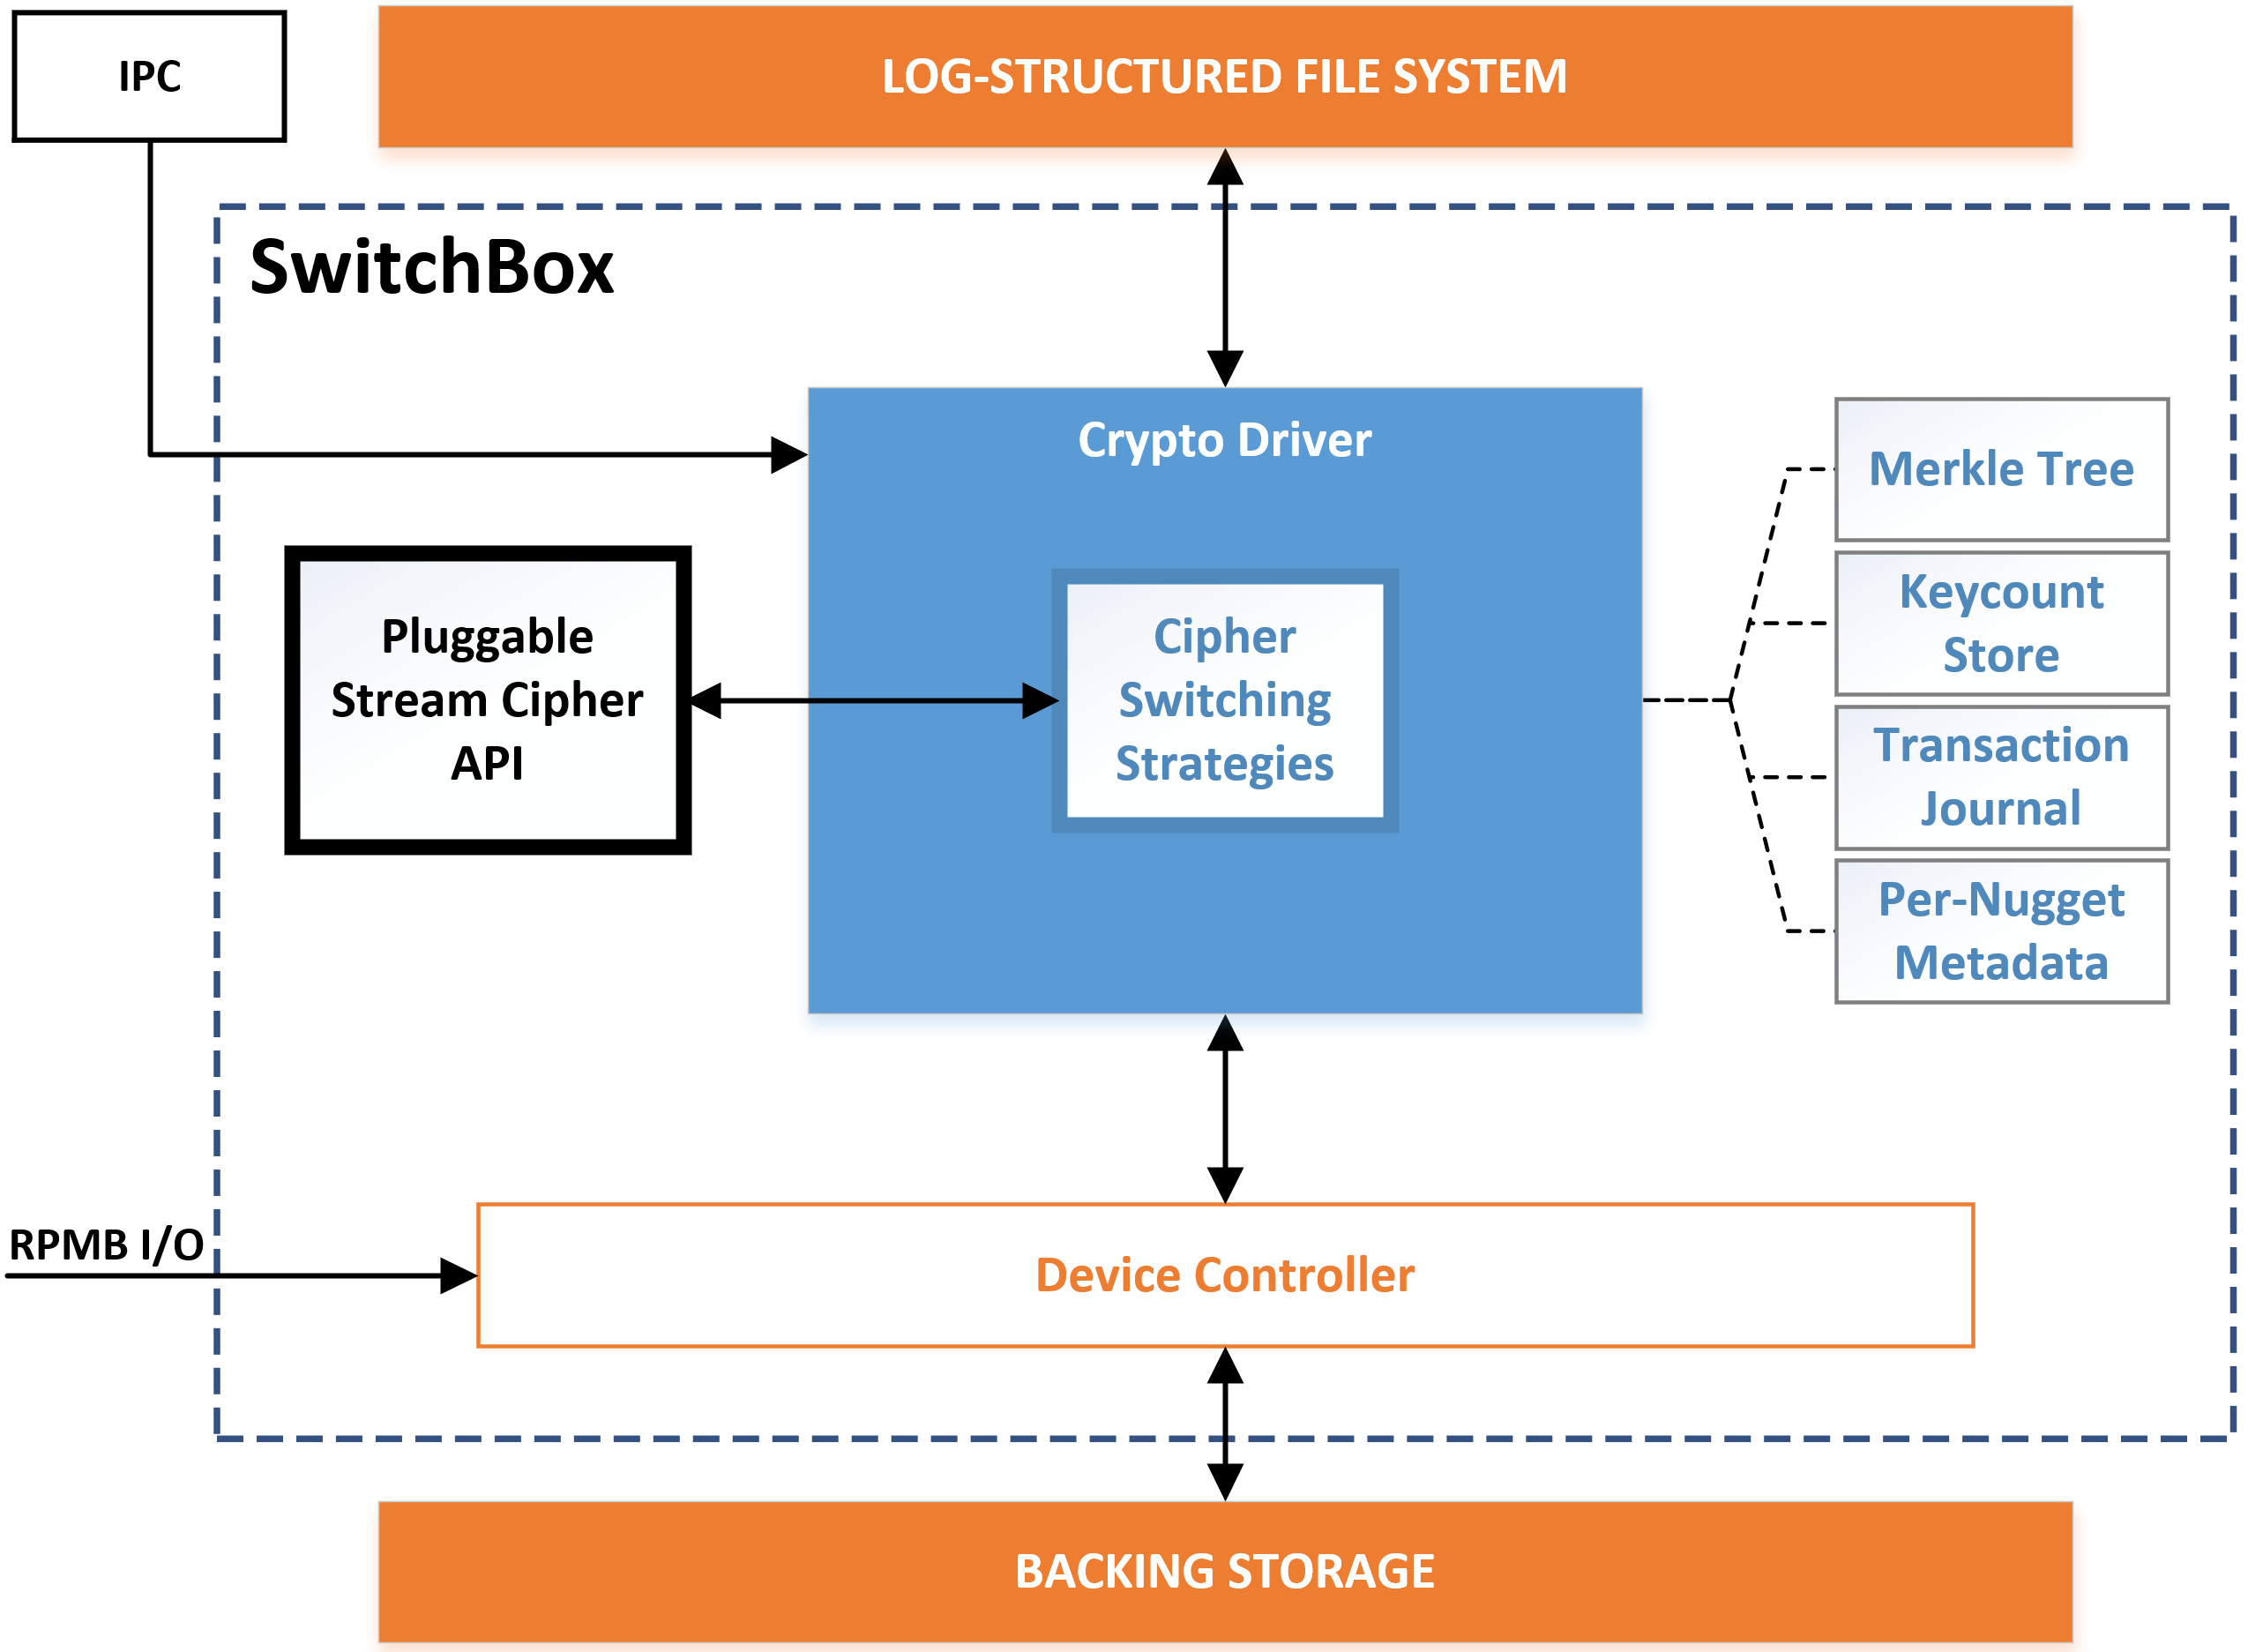
\includegraphics[width=\linewidth]{overview.png}
   \caption{Overview of the SwitchBox construction.}\label{fig:overview}
\end{figure}

In this section, we describe our mechanism to navigate the cipher configuration
space and cipher switching strategies. We also discuss the pluggable stream
cipher API and other design challenges.

SwitchBox is a translation layer ideally implemented in the Flash Translation
Layer (FTL). Unlike prior work, which focuses on optimizing performance despite
re-keying due to overwrites, SwitchBox maintains overwrite protections while
abstracting the idea of re-keying out into re-ciphering or \emph{cipher
switching}, where a nugget's contents are decrypted using the old key and
inactive cipher configuration and encrypted using a new key and the active
cipher configuration before completing the I/O operation; instead of myopically
pursuing a performance win, this allows us to trade off different ciphers and
their characteristics online.

\begin{figure}[t]
\centering
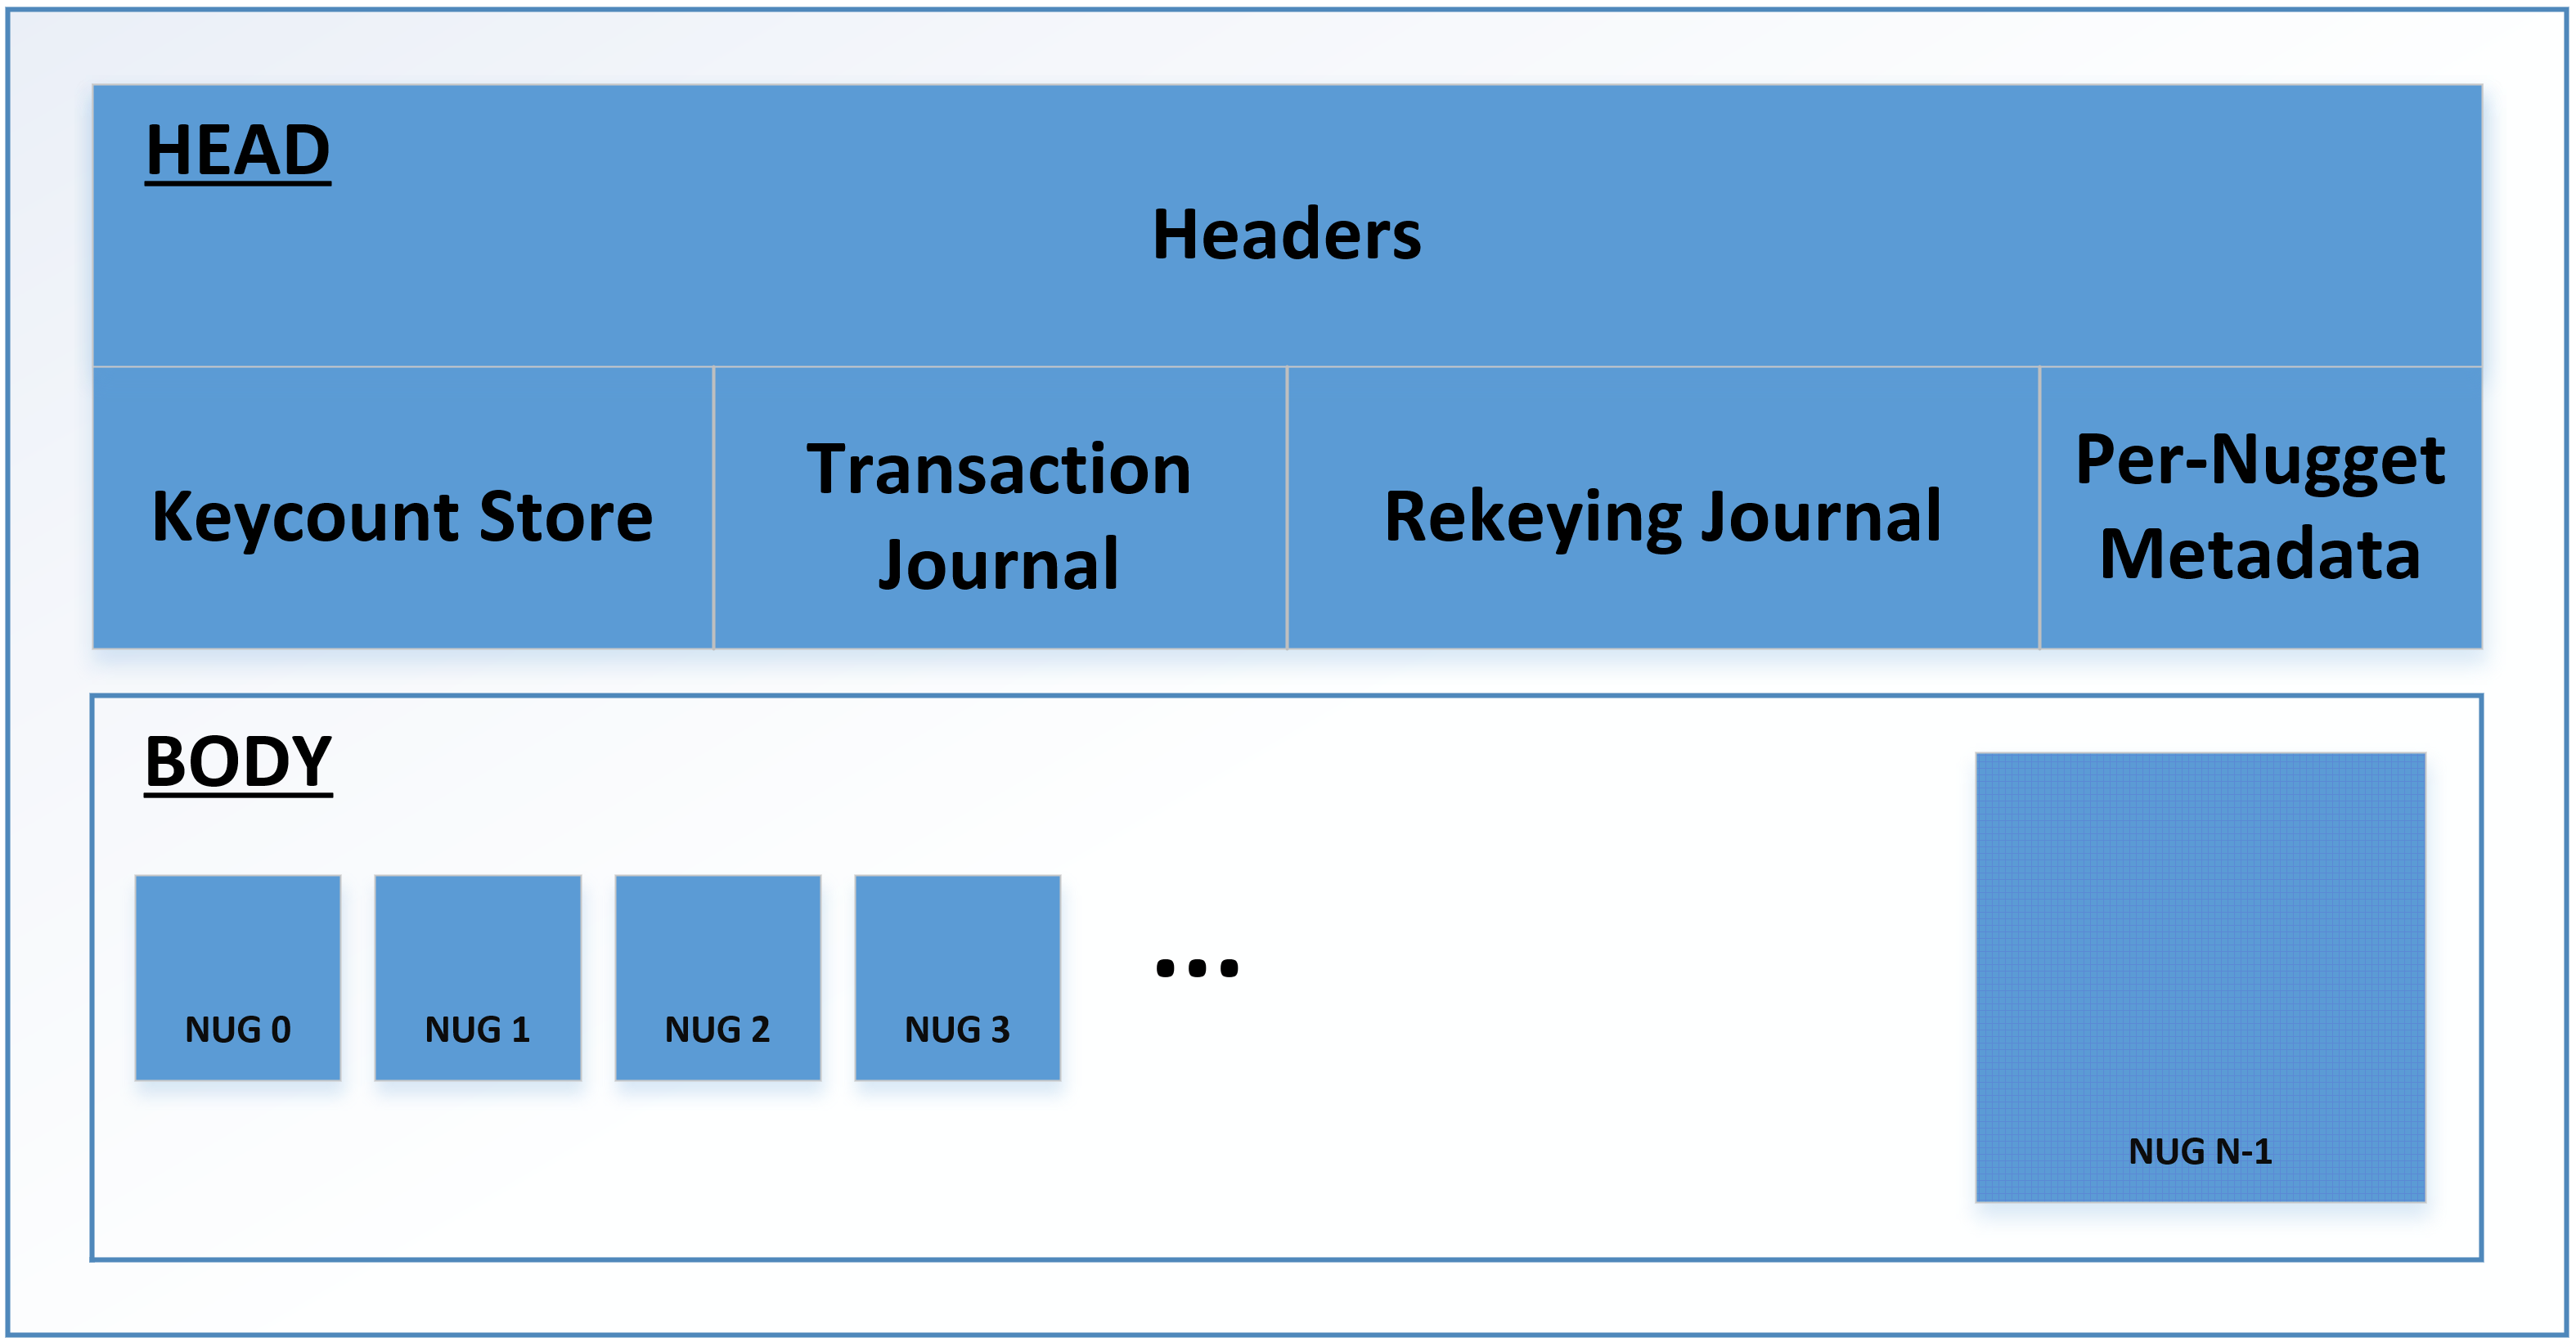
\includegraphics[width=\linewidth]{backstore.png}
 \caption{Layout of SwitchBox's backing storage.}\label{fig:backstore2}
\end{figure}

The backing store is the storage medium SwitchBox operates on. The layout of the
backing store is illustrated in \figref{backstore2}. In the \textit{body}
section of the backing store layout, end-user data is partitioned into a series
of same-size \emph{logical blocks} marked \textit{NUG} for \emph{nugget}. A
nugget consists of one or more physical drive blocks and per-nugget metadata
indicating which cipher was used to encrypt the nugget. We borrow this
terminology from prior work to easily differentiate our logical blocks (nuggets)
from physical drive and other storage blocks.

\figref{overview} provides an overview of the SwitchBox design. SwitchBox
manages five metadata components: an in-memory \emph{Merkle Tree}; two
drive-backed byte arrays, \ie{the \emph{Keycount Store} and the
\emph{Transaction Journal}}; a globally persistent cryptographically secure
monotonic counter; and a flexible drive-backed store for cipher-specific
\emph{per-nugget metadata}.

These five components are tightly integrated into the cryptographic driver,
which handles data encryption, decryption, overwrite detection, integrity
protection, IPC with the wider system to determine the active cipher
configuration, and the execution of cipher switching strategies with stream
cipher implementations provided by a pluggable stream cipher API. The
cryptographic driver interacts with 1) the overlying LFS through traditional I/O
passed through the Linux Virtual Filesystem Switch (VFS) and 2) the underlying
drive through the device controller block I/O layer or as part of the FTL,
depending on implementation.

\subsection{Pluggable Stream Cipher API}

We develop an API to allow any stream cipher or any cipher that can operate as a
stream cipher to be used with SwitchBox without modification or special
considerations. In this way, different stream ciphers might appear to all be
interchangeable, but they are not. For instance: not all stream ciphers, let
alone all ciphers, are length-preserving. A length-preserving cipher generates
ciphertext output of the same length as its plaintext input, \eg{ChaCha20}. A
cipher like Freestyle, on the other hand, is not length-preserving and has the
overhead of additional cryptographic material that must be stored and indexed
alongside any generated ciphertext. Hence, we built SwitchBox as a novel common
cipher interface that allows ciphers with entirely disparate output
characteristics to co-exist on the same drive; typically, such characteristics
would render these ciphers entirely incompatible, preventing us from trading
them off with one another.

SwitchBox exposes hooks for wrapper functions at three levels:

\begin{itemize}
   \item \textbf{\texttt{sc\_fn\_crypt\_data}}\\\texttt{sc\_fn\_crypt\_data}
   expects a cipher to accept intra- and inter- nugget offset data and return
   crypted the specified region and so operates at a fine-grain level compared
   to using the read and write handles described below. There is no distinction
   made between encryption and decryption as they're considered the same
   operation in this context. Further, this interface does not allow any access
   to the SwitchBox internals and is expected to execute independently of
   SwitchBox.

   Unlike \texttt{sc\_fn\_crypt\_data\_custom},
   \\\texttt{sc\_fn\_crypt\_data} performs the final XORing automatically,
   returning a convenient xor buffer to read crypted data into. As such, it
   provides a slightly higher level of interaction with the backing store's data
   making things easier for simpler ciphers.
   \item \textbf{\texttt{sc\_fn\_crypt\_data\_custom}}\\Unlike
   \texttt{sc\_fn\_crypt\_data}, \\\texttt{sc\_fn\_crypt\_data\_custom} does not
   perform the final XORing automatically, nor does it provide the convenient
   xor buffer to deal with crypted data automatically, for ciphers that require
   this functionality. As such, it provides a slightly lower level of
   abstraction when accessing to the backing store.
   \item \texttt{sc\_fn\_read\_handle} and \texttt{sc\_fn\_write\_handle}\\
   Unlike the other two levels, both hooks must be provided by a cipher or
   functionality is undefined. At this level, control over encryption is
   coarse-grain, where cipher wrappers have access to all relevant SwitchBox
   internals and must implement cipher switching manually.
   \texttt{sc\_fn\_read\_handle} expects a cipher to accept a buffer and read
   into it a decrypted subset of a nugget's ciphertext.

   \texttt{sc\_fn\_write\_handle} expects a cipher to accept
   some plaintext buffer and commit some encrypted subset of the current nugget
   to the backing store.

   This is a good choice if a cipher with randomized output needs to work below
   the overwrite protection code (\ie{Freestyle}) and/or a cipher doesn't
   function like a stream cipher (\ie{AES-XTS}). If
   \texttt{sc\_fn\_read\_handle} is defined, \\\texttt{sc\_fn\_write\_handle}
   must also be defined. Hooks at this level should only ever operate on a
   single nugget or SwitchBox behavior is undefined. Further, due to cipher
   swapping, this function must not read in any nugget/flake data from the
   backstore if a perfectly aligned nugget-sized chunk is requested. This is
   because this API hook may be called when cipher switching and the underlying
   data in the nugget might be crypted with a different algorithm when
   attempting to read it, corrupting the plaintext.
\end{itemize}

\subsection{Cipher Switching Strategies}

At any moment, the currently active cipher configuration is used to encrypt
nugget contents. Until the wider system indicates that SwitchBox should use a
different cipher to interact with the backing store, the active cipher
configuration is used to encrypt and decrypt all nuggets during I/O.

When the wider system determines a cipher switch should occur for whatever
reason, it is entirely non-trivial to determine \emph{when} to encrypt a nugget
with a different cipher and \emph{where} to direct the output of that cipher.
Depending on the complexity of the use case, it may make the most sense to
re-cipher a nugget immediately, or eventually, or to re-cipher a series of
nuggets. A simple approach would immediately switch every nugget in the backing
store to the desired cipher, but the cost of doing that conversion would likely
consume more energy than would be saved in future accesses; the egregious
latency penalty incurred waiting for the entire drive to be re-ciphered would be
similarly unacceptable.

Hence, a more strategic approach and adaptable is necessary: cipher switching
\emph{strategies}. These strategies are an essential part of the mechanism by
which SwitchBox can efficiently transition nuggets between different encrypted
states without egregious penalties to latency or battery life, thus providing a
realistic mechanism to navigate our cipher configuration tradeoff space.

Determining \emph{when} to target a nugget for re-ciphering we call
\emph{temporal switching}, for which we propose the \emph{Forward} switching
strategy and its variants. Determining \emph{where}---in which partition and
across which nuggets--to output ciphertext we call \emph{spatial switching} for
which we propose the \emph{Mirrored} and \emph{Selective} switching strategies.
Each comes with various security, performance, and energy trade offs.

\tblref{strategies-advantages} summarizes the various advantages and
disadvantages of these strategies and each strategy and is explained more below.

\subsubsection{Forward Switching Strategy}

SwitchBox allows each individual nugget to exist encrypted with any cipher the
pluggable cipher API makes available regardless of the currently active cipher
configuration. When a nugget is encountered during I/O that is encrypted using a
cipher other than the active cipher configuration, the Forward strategy dictates
that this nugget be re-ciphered immediately. If a particular nugget encrypted
with a non-active cipher configuration is never encountered during I/O, it is
never re-ciphered and remains on the backing store in its original state. In
this way, the Forward strategy represents a form of temporal cipher switching.

Rather than re-cipher the entire backing store every time the active cipher
configuration changes, this strategy limits the performance impact of cipher
switching to individual nuggets. Similar to ``re-keying'' in prior
work~\cite{StrongBox}, the heavy price of re-ciphering is paid only once, after
which the nugget is accessed normally during I/O until the active cipher
configuration is switched again.

\PUNT{There are several forms the Forward strategy might take. The default and most
intuitive is \emph{0-forward}, in which SwitchBox immediately transitions
individual nuggets encountered during I/O to the active cipher configuration if
they are not using it. Over time, if various I/O operations end up touching
every nugget in the backing store, the encrypted contents of every nugget will
become decryptable with the currently active cipher configuration.

The Forward strategy might also take the form of \emph{N-forward}, where SwitchBox
attempts to take advantage of spatial sequential locality to transition whole
sets of nuggets into the active cipher configuration. We can trivially expand
the forward strategy to encompass the entire backing store by selecting $N$
equal to the total number of nuggets managed by SwitchBox. This would have the
overhead of re-ciphering large swaths of the backing store upon every I/O
operation where a nugget encrypted with the non-active cipher configuration is
encountered. Of course, this has the same dire implications for performance as
simply re-initializing the entire filesystem or encrypted container with the new
cipher.}

\subsubsection{Selective Switching Strategy}

When SwitchBox is initialized with the Selective strategy, the backing store is
partitioned into $C$ regions where $C$ represents the number of ciphers in use;
each region's nuggets are encrypted by each of the $C$ ciphers respectively. For
instance, were SwitchBox initialized using two ciphers ($C = 2$), the backing
store would be partitioned in half; all nuggets in the first partition would be
encrypted with the first cipher while all nuggets in the second partition would
be encrypted with the second.

Hence, unlike the Forward strategy, which schedules individual nuggets to be
re-ciphered at some point in time \emph{after} the active cipher configuration
is switched, the Selective strategy allows the wider system to indicate
\emph{where} on the backing store a read or write operation should occur. In
this way, the selective strategy represents a form of spatial cipher switching
where different regions of the backing store can store different pieces of data
encrypted with different ciphers.

\subsubsection{Mirrored Switching Strategy}

Similar to the Selective strategy, when SwitchBox is initialized with the
Mirrored strategy, the backing store is partitioned into $C$ regions where $C$
represents the number of ciphers in use; each region's nuggets are encrypted by
each of the $C$ ciphers respectively. The nuggets in each partition are
encrypted with their respective ciphers.

However, unlike the Selective strategy, all write operations that hit one
partition are mirrored into the other partitions immediately. The mirrored
strategy allows the wider system to indicate where on the backing store a
\emph{read} operation should occur. In this way, the Mirrored strategy, like the
Selective strategy, represents a form of spatial cipher switching. All regions
of the backing store will always be in a consistent state and share the same
data.

\subsection{Cipher Switching: A Mechanism To Re-Cipher A Nugget}

Having cipher switching strategies by themselves is not enough to facilitate
cipher switching. We require some mechanism to navigate the
latency/energy/security tradeoff space of cipher configurations through applying
these strategies. Where a naive implementation is trivial (\eg{execute the
chosen strategy on every I/O operation}), this navigation must occur with
acceptable overhead by preserving performance wherever possible. The
cryptographic driver provides such a mechanism, tying together cipher switching
strategies and the pluggable stream cipher API.

In the cases of Mirrored and Selective switching, we use offset to determine in
which area of the backing store receives I/O.

In the case of Forward switching, it is tempting to implement it such that a
nugget is completely re-ciphered during I/O every time its metadata indicates
that it was previously encrypted using a non-active cipher. However, such a
naive implementation can have disastrous effects on performance depending on the
workload.

First, a nugget is considered \emph{pristine} if it has not had any data written
into it yet. SwitchBox determines if a nugget is pristine by checking the state
of the transaction journal for that nugget. A pristine nugget will have a clean
transaction journal.

All nuggets start out as pristine. All nuggets start out with metadata
indicating that they're to be encrypted and decrypted by the initially active
cipher. This is true \emph{even if the nugget has not been written to yet}. This
means, on read and write operations after a different cipher becomes the active
cipher configuration using a naively implemented forward switching strategy,
every write operation will trigger a re-keying, which carries significant
overhead.

The solution is to divide forward switching into \emph{soft re-ciphering} and
\emph{hard re-ciphering}. Fortunately, the SwitchBox design lends itself nicely
to such a distinction for free, as per-nugget metadata is managed separately
from a nugget's actual data.

During soft re-ciphering, only the nugget's metadata is changed to indicate that
the nugget can be encrypted and decrypted with the newly active cipher
configuration but \emph{without actually re-ciphering the nugget data itself}.
This keeps the nugget in its pristine condition, preserving SwitchBox's ability
to write data into it without triggering a costly re-keying operation every
time, preserving our performance advantage. At the same time, SwitchBox can now
use the newly active cipher configuration to interact with the nugget as
expected. On the other hand, during hard re-cipher, the nugget's metadata is
changed to match the active cipher configuration \emph{and} the nugget data is
encrypted using the new cipher.

\PUNT{When using forward switching other that 0-forward, \ie{N-forward} where $N
> 0$, only read operations are allowed to trigger hard re-ciphering for nuggets
other than the currently active nugget. This is still not enough to preserve our
performance advantage, however, as I/O operations can span multiple nuggets, and
attempting to take advantage of spatial locality after interacting with every
nugget is counterproductive. Hence, only the last nugget touched by a read
operation will trigger the more aggressive N-forward behavior if $N > 0$. These
considerations have the effect of 1) preserving our performance advantage and 2)
allowing more aggressive N-forward behavior (where $N > 0$) to take advantage of
spatial locality during read-heavy workloads to result in a further performance
advantage (see: \secref{evaluation}).}

\subsection{Comparing Cipher Switching Strategies}

\begin{table}[]
   \begin{tabular}{@{}|l|l|l|l|@{}}
      \toprule
      \textbf{Strategy} & \textbf{Convergence} & \textbf{Waste} & \textbf{Performance} \\ \midrule
      Forward   & Slow           & Low  & Workload dependent    \\
      \hline
      Mirrored  & Nearly instant & High & Fast read; slow write \\
      \hline
      Selective & Impossible     & High & Fast read and write   \\
      \hline
   \end{tabular}
   \caption{A summary comparison between the three cipher switching strategies.
   \emph{Convergence} represents the amount of time it takes to switch the
   entire backing store to a single cipher configuration using one strategy.
   \emph{Waste} represents a strategy's impact on the amount of free space
   reported to the OS. \emph{Performance} represents the performance impact a
   strategy has on read and write throughput.}
   \label{tbl:strategies-advantages}
\end{table}

\tblref{strategies-advantages} summarizes the tradeoffs between the three cipher
switching strategies. In order:

\textbf{Convergence:} Depending on the use case, the ability to quickly
converge the entire backing store to a single cipher configuration is very
useful (see: \secref{usecases}); \eg{switching to a cipher low energy
configuration optimized when battery state becomes critical or when certain
other security properties become more desirable}. The near-instantaneous nature
of SSD Instant Secure Erase (ISE) implementations on modern
SSDs~\cite{ISE1,ISE2,ISE3} makes this a very fast process for the Mirrored
strategy. Since the Forward strategy is unlikely to switch every nugget in the
backing store after a cipher switch, depending on the workload, it may not
require cipher switching on every nugget. In the best case, only a small handful
of high traffic nuggets will require re-ciphering. In the worse case, every
nugget on the drive will require re-ciphering, which would be slow. This makes
the Forward strategy slow to converge compared to Mirrored, but the nugget
cipher configurations can be made consistent eventually. Unlike the other
strategies, the Selective strategy is structurally required to maintain multiple
encrypted partitions, which makes converging the entire drive's nuggets to one
cipher configuration impossible.

\textbf{``Waste'':} Unlike the other two strategies, using
the Forward strategy does not dramatically reduce the total usable space on the
drive by the end-user. This is because the Forward strategy allows nuggets with
various cipher configurations to co-exist contiguously on the backing store.
Since the Mirrored and Selective strategies require partitioning the backing
store into some number of partitions---where the filesystem size reported back
to the OS is some function of partition size---there is a necessary reduction in
usable space.

\textbf{Performance:} The Selective and Mirrored strategies can read data
from the backing store with low overhead, reaching performance parity with prior
work. This is because switching ciphers using these strategies amounts to
offsetting the read index so it lands in the proper partition, which has little
overhead. The Forward strategy also reads with low overhead except in the case
where the current nugget was not encrypted with the active cipher configuration.
This triggers re-ciphering, which can be costly if the workload touches unique
nuggets while executing, \ie{long sequential writes vs write-once read-many}.

The Selective strategy also writes with low overhead because, like with reads,
an offset is the only requirement. The Mirrored strategy, on the other hand, can
be two or more times slower for writes (when $C = 2$) compared to baseline. Each
additional partition ($C > 2$) compounds the write penalty. This is because each
writes is ``mirrored'' across all partitions. As with reads, the Forward
strategy writes with low overhead except in the case where the current nugget is
not pristine and was not encrypted with the active cipher configuration. This
triggers costly re-ciphering, which can compound depending on workload.

\subsection{Threat Model for Cipher Switching Strategies}

The primary concern facing any FDE solution is that of confidentiality: an
adversary should not be able to decrypt encrypted plaintext without the right
key. With this research, we select five cipher implementations and configure
them under Switchbox: ChaCha~\cite{ChaCha20} (ChaCha8 and ChaCha20), and
Freestyle~\cite{Freestyle}. Each cipher has been proven formally secure in that
there are no known efficient attacks against them. Any such cipher can be used
with SwitchBox.

Encryption is achieved via a binary additive approach: cipher output (keystream)
is combined with plaintext nugget contents using XOR, with metadata to track
writes and ensure that pad reuse never occurs during overwrites and that the
system can recover from crashes into a secure state~\cite{StrongBox}.

Another concern is data integrity: an adversary should not be able to tamper
with ciphertext and it go unnoticed. As with prior work, we use an in-memory
Merkle Tree to ensure nugget and system integrity~\cite{StrongBox}.

Switching strategies add an additional concern: even if we initiate a ``cipher
switch,'' there may still be data on the drive that is encrypted with a
non-active cipher configuration. Is this a problem? For the Forward strategy,
this implies data may at any time be encrypted using the least desirable cipher.
For the Mirrored and Selective strategies, the backing store is partitioned into
regions where nuggets are guaranteed to be encrypted with each cipher. However,
in terms of confidentiality, all the ciphers we configured under SwitchBox have
been proven formally secure. Hence, nuggets encrypted with different secure
ciphers can co-exist on the backing store securely, depending on the use case
(see: \secref{usecases}).

\subsection{A Relative Scoring of Cipher Security Properties}

Every cipher mentioned in this paper has been proven formally secure in that
\emph{there are no known efficient attacks against any of them}~\cite{All,
Ciphers, Again}. This implies data is kept confidential versus an adversary with
limited resources, however it is often desirable to secure data at rest in
special contexts or considering future adversaries with abundant resources at
their disposal. In this way, a cipher that is more resilient to cryptanalysis or
brute-force than is currently required might be more desirable than a cipher
with properties that meet current standards, \eg{future-proofing storage}.

To simplify reasoning about trading off such disparate cryptographic properties
in the FDE context, we must have a way to quantitatively compare a cipher's
``desirability'' or usefulness to SwitchBox and to FDE more generally. Hence, we
do not attempt to define a generally applicable \textit{ranking} of
\emph{security strength} as that doesn't make sense. Instead, we score ciphers
(\ie{a so-called ``security score''}) based on three key security properties
that, when summed, give an estimate of the usefulness of a cipher to SwitchBox
FDE (see: \tblref{security-quant}).

The scores we use are a combination of schemes that are already well understood:
scoring ciphers on their confusion and diffusion of plaintext bits during
encryption~\cite{MicrosoftCryptanalysisAES,SchneiersOnRounds} (\ie{round
count}), scoring ciphers on how they behave when given the same input
parameters~\cite{random-output1,Freestyle,random-output2} (normally an
unacceptable confidentiality-breaking overwrite condition), and asymmetric
penalties for supplying the wrong key when attempting to decrypt nugget
ciphertext (\ie{an attacker should have to do more work than the
defender})~\cite{scrypt,Freestyle,others2}.\\
\\
\textbf{1) Output randomization (OR).} A cipher with output randomization
generates different ciphertexts non-deterministically given the same key, nonce,
and message. This makes chosen-ciphertext (CCA) and other attacks where the
ciphertext is in full control of the adversary much more difficult.

This is a binary feature in that a cipher either outputs deterministically given
the same input or it does not. A cipher with non-deterministic output given the
same key, nonce, and message as inputs scores a 1 for this feature while a
cipher with deterministic output given the same input scores a 0.\\
\\
\textbf{2) Resistance to brute force and offline/dictionary attacks (RBF).}
All the ciphers we consider are resistant to ciphertext-only brute force and
dictionary attacks, which is paramount for the encryption of data at rest. We
narrowly define ``standard resistance'' versus brute-force and
offline/dictionary attacks with respect to the time taken to finish decrypting
ciphertext given an incorrect key versus a correct key; a cipher with standard
resistance to brute force and offline/dictionary attacks has no kind of
\emph{key-guessing penalty}~\cite{Freestyle}---the ciphertext is decrypted no
slower when given the incorrect key versus the correct key. Similarly, we
consider ciphers with so-called ``enhanced resistance,'' where they are expected
to take longer to finish decrypting ciphertext given an incorrect key versus a
correct key with high probability.

Scores for this feature range from 0 to 1, where 0 represents no resistance, 0.5
represents standard resistance to brute-force and offline/dictionary attacks,
and 1 represents enhanced resistance.\\
\\
\textbf{3) Relative round count and key length (RR/RK).} The ciphers we examine
in this research are all constructed around the notion of \emph{rounds}, where a
higher number of rounds typically implies a stronger confidentiality guarantee
given there are no fatal related-key attacks. This feature represents how many
rounds the cipher executes compared to the accepted ``standard'' round count for
that cipher. For instance, ChaCha8 is a reduced round version of the standard
ChaCha20. Variants are distributed evenly from 0-1. For instance, ChaCha8 scores
0 and ChaCha20 scores 1\@.

\begin{table}[]
  \begin{tabular}{@{}lllll@{}}
  \toprule
  \textbf{Cipher} & \textbf{OR} & \textbf{RBF} & \textbf{RR/RK} & \textbf{score} \\ \midrule
  ChaCha8         & 0           & 0.5          & 0              & 0.5            \\
  %ChaCha12        & 0           & 0.5          & 0.5            & 1              \\
  ChaCha20        & 0           & 0.5          & 1              & 1.5            \\
  %Salsa8          & 0           & 0.5          & 0              & 0.5            \\
  %Salsa12         & 0           & 0.5          & 0.5            & 1              \\
  %Salsa20         & 0           & 0.5          & 1              & 1.5            \\
  %AES128-CTR      & 0           & 0.5          & 0              & 0.5            \\
  %AES256-CTR      & 0           & 0.5          & 1              & 1.5            \\
  %HC128           & 0           & 0.5          & 0              & 0.5            \\
  %HC256           & 0           & 0.5          & 1              & 1.5            \\
  Freestyle (F)   & 1           & 1            & 0              & 2              \\
  Freestyle (B)   & 1           & 1            & 0.5            & 2.5            \\
  Freestyle (S)   & 1           & 1            & 1              & 3
  \end{tabular}
  \caption{\TODO{Table caption goes here.}}
  \label{tbl:security-quant}
\end{table}
